\documentclass[11pt,a4paper]{article}
\usepackage{fontspec}
\usepackage{xeCJK}
\setCJKmainfont{SimSun}
\setCJKsansfont{Microsoft YaHei}
\setCJKmonofont{SimSun}
\usepackage[margin=1.85cm]{geometry}
\usepackage{xcolor}
\usepackage{tikz}
\usetikzlibrary{arrows.meta,positioning,calc}
\usepackage{booktabs}
\usepackage{tabularx}
\usepackage{array}
\usepackage{enumitem}
\usepackage{fancyhdr}
\usepackage{hyperref}
\usepackage{listings}
\usepackage{amsmath}
\usepackage{amssymb}

\definecolor{navy}{HTML}{17365D}
\definecolor{blue}{HTML}{2F75B5}
\definecolor{lightblue}{HTML}{EEF5FA}
\definecolor{green}{HTML}{548235}
\definecolor{lightgreen}{HTML}{EEF6EA}
\definecolor{orange}{HTML}{C55A11}
\definecolor{lightorange}{HTML}{FFF3E8}
\definecolor{red}{HTML}{A61B1B}
\definecolor{gray}{HTML}{5B6573}
\definecolor{lightgray}{HTML}{F4F6F8}

\hypersetup{colorlinks=true,linkcolor=blue,urlcolor=blue}
\setlength{\parindent}{0pt}
\setlength{\parskip}{4pt}
\setlist[itemize]{leftmargin=1.5em,itemsep=2pt,topsep=3pt}
\setlist[enumerate]{leftmargin=1.7em,itemsep=2pt,topsep=3pt}
\setlength{\emergencystretch}{3em}
\sloppy

\pagestyle{fancy}
\fancyhf{}
\setlength{\headheight}{14pt}
\fancyhead[L]{\textcolor{gray}{Tri-EvoBench | Final Matrix Analysis}}
\fancyhead[R]{\textcolor{gray}{2026-09-11}}
\fancyfoot[C]{\textcolor{gray}{\thepage}}

\newenvironment{callout}{\begin{quote}\small\color{navy}}{\end{quote}}
\newcommand{\code}[1]{\texttt{#1}}
\newcommand{\passrate}[1]{\textbf{#1\%}}

\title{\vspace{-1.2cm}\textcolor{navy}{Tri-EvoBench}\par\vspace{4pt}\Large 三类自进化智能体正式评测分析}
\author{项目组}
\date{2026 年 9 月 11 日}

\begin{document}
\maketitle
\thispagestyle{empty}

\begin{center}
\textcolor{gray}{Hermes、SkillOpt、Trace2Skill 在 L1/L2 长流上的统一 Docker 评测结果}
\end{center}

\vspace{6pt}
\begin{callout}
本轮完成 87 个 stream-agent 任务、1,671 个 agent-turn。结果表明：在 L1 上，SkillOpt 与 Hermes 的严格通过率几乎持平，但 SkillOpt 以约一半的 token/turn 获得更高平均分；在 L2 上，Hermes 的平均分和通过率均领先。Trace2Skill 在两个层级都显著落后，同时产生最多的 API calls/turn，说明“从轨迹抽取技能”的学习链已经接通，但尚未稳定转化为当前任务分布上的执行收益。
\end{callout}

\section{评测对象与规模}

本报告分析的是同一模型配置、同一 Runner 生命周期和同一 Docker 隔离条件下的三种自进化 Agent。模型统一为 \code{deepseek-v4-flash}，运行配置关闭 thinking。所有正式任务均在服务器 Docker 环境中执行；模型输出、工具轨迹、工作区快照、Judge 结果和演化记录均落盘。

\begin{center}
\renewcommand{\arraystretch}{1.25}
\begin{tabularx}{0.98\linewidth}{>{\bfseries}p{0.16\linewidth}p{0.16\linewidth}p{0.14\linewidth}X}
\toprule
层级 & Streams & Turns/Agent & 主要能力压力 \\
\midrule
L1 Arena & 23 & 423 & 持久工作区、跨轮状态、动态更新、偏好约束、噪声回合、代码与文档副作用。平均 18.39 turns/stream。\\
L2 Demo V2 & 6 & 134 & 数据分析、代码生成、可视化、文本推断、工具策略与原生私有验证。包含一条 100-turn SRA 长流。\\
\midrule
总计 & 29 & 557/Agent & 三个 Agent 合计 87 个 stream-agent 任务、1,671 turns。\\
\bottomrule
\end{tabularx}
\end{center}

L2 的六条流覆盖 AIRS 文本蕴含（2 turns）、MLGym Titanic（2 turns）、SkillLearn 股票可视化（10 turns）、SkillsBench data-to-D3（10 turns）、SRA BigCodeBench Pandas 可视化（100 turns）和 Tau2 电信漫游（10 turns）。这使 L2 同时包含短任务和极长连续任务，不只是 smoke test。

\section{成品评测流程}

\begin{center}
\begin{tikzpicture}[node distance=6mm and 5mm, >=Latex, every node/.style={font=\scriptsize},
  core/.style={rounded corners=2pt, draw=navy, fill=lightblue, minimum height=12mm, text width=28mm, align=center},
  base/.style={rounded corners=2pt, draw=green!70!black, fill=lightgreen, minimum height=12mm, text width=27mm, align=center},
  eval/.style={rounded corners=2pt, draw=orange!80!black, fill=lightorange, minimum height=12mm, text width=29mm, align=center}]
\node[core] (stream) {Benchmark Stream\\有序 Turn + 持久状态};
\node[core, right=of stream] (runner) {Tri-EvoBench Runner\\预算、隔离、断点};
\node[base, right=of runner] (agent) {Agent Bridge\\Hermes / SkillOpt / Trace2Skill};
\node[eval, right=of agent] (judge) {Docker Sandbox\\原生 Verifier + Judge};
\node[eval, below=of agent] (evo) {Evolution Barrier\\只接收公开轨迹与反馈};
\node[core, below=of runner] (evidence) {summary + trace + checkpoint\\usage + state hash};
\draw[->, thick, navy] (stream) -- (runner);
\draw[->, thick, navy] (runner) -- (agent);
\draw[->, thick, navy] (agent) -- (judge);
\draw[->, thick, orange!80!black] (judge) |- (evo);
\draw[->, thick, orange!80!black] (evo) -- (evidence);
\draw[->, thick, navy] (evidence) -- (runner);
\end{tikzpicture}
\end{center}

每个 Turn 经过 \code{start\_turn -> interact -> judge/verifier -> evolve -> checkpoint}。当一次交互失败但允许反馈重试时，Runner 只追加新的 Interaction；当网络或评测进程在第 $n+1$ 个 Turn 中断时，系统恢复第 $n$ 个 Turn 后的精确 checkpoint，只重跑尚未完成的部分。L2 还支持保存“Agent 已返回、Judge 尚未完成”的 post-agent checkpoint，从而避免为重新裁决再次调用付费 Agent。

\subsection*{三种 Agent 如何融入同一生命周期}

\begin{center}
\small
\renewcommand{\arraystretch}{1.28}
\begin{tabularx}{0.99\linewidth}{>{\bfseries}p{0.12\linewidth}>{\raggedright\arraybackslash}X>{\raggedright\arraybackslash}X>{\raggedright\arraybackslash}X}
\toprule
维度 & Hermes & SkillOpt & Trace2Skill \\
\midrule
运行入口 & Docker process adapter，复用 SessionManager/\allowbreak AIAgent & NDJSON bridge，连接 target backend & NDJSON bridge，运行 CLIOnly/\allowbreak CLISkillPreloaded agent \\
持久学习态 & memory、skills 与 session state & \code{skill.md}、history 与 skill hash & \code{skills/}、history、trajectory 与 patch \\
演化阶段 & native/background review 或 turn barrier & Reflect $\to$ Aggregate $\to$ Clip $\to$ Update & MAP $\to$ REDUCE $\to$ APPLY $\to$ VERIFY \\
公开证据 & 回复、动作、工具、事件、状态、usage & 回复、文件动作、skill 变化、usage & 真实工具步骤、观察、skill/\allowbreak evolution 文件、usage \\
隔离边界 & \multicolumn{3}{>{\raggedright\arraybackslash}p{0.79\linewidth}}{私有 verifier/oracle 不进入 Agent；Interaction 期间冻结学习文件，学习只能在 evolution barrier 发生。} \\
\bottomrule
\end{tabularx}
\end{center}

\section{最终结果矩阵}

\begin{center}
\renewcommand{\arraystretch}{1.25}
\setlength{\tabcolsep}{8pt}
\begin{tabular}{llrrrrr}
\toprule
层级 & Agent & Turns & 通过 & 通过率 & Mean score & Tokens \\
\midrule
L1 & Hermes & 423 & 265 & 62.65\% & 0.6875 & 153.52M \\
L1 & SkillOpt & 423 & \textbf{266} & \textbf{62.88\%} & \textbf{0.7478} & \textbf{76.56M} \\
L1 & Trace2Skill & 423 & 70 & 16.55\% & 0.2260 & 102.56M \\
\midrule
L2 & Hermes & 134 & \textbf{49} & \textbf{36.57\%} & \textbf{0.4746} & 82.82M \\
L2 & SkillOpt & 134 & 42 & 31.34\% & 0.4142 & \textbf{50.25M} \\
L2 & Trace2Skill & 134 & 9 & 6.72\% & 0.2007 & 58.45M \\
\bottomrule
\end{tabular}
\end{center}

\subsection*{严格通过率对比}

\begin{center}
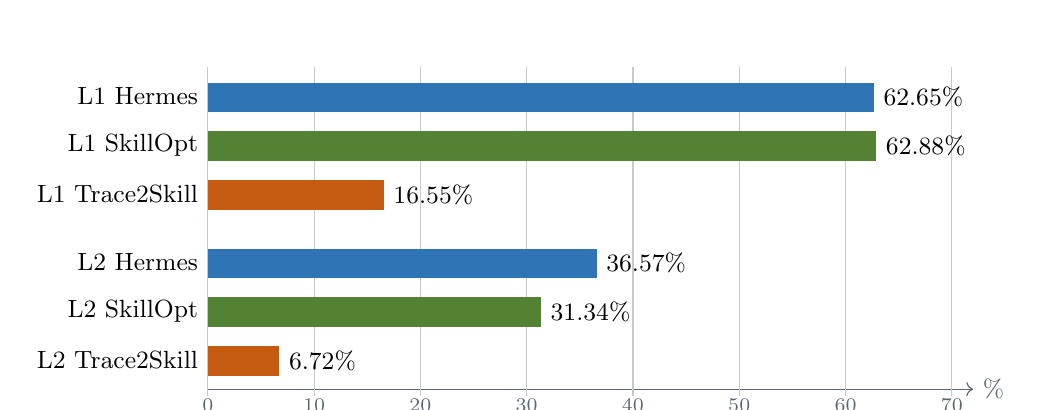
\begin{tikzpicture}[x=0.135cm,y=0.62cm,font=\small]
\draw[->,gray] (0,0) -- (72,0) node[right]{\%};
\foreach \x in {0,10,...,70} {\draw[gray!35] (\x,-0.15)--(\x,6.6); \node[below,gray] at (\x,0){\scriptsize \x};}
\node[left] at (0,6){L1 Hermes};       \fill[blue]   (0,5.68) rectangle (62.65,6.28); \node[right] at (62.65,5.98){62.65\%};
\node[left] at (0,5){L1 SkillOpt};     \fill[green]  (0,4.68) rectangle (62.88,5.28); \node[right] at (62.88,4.98){62.88\%};
\node[left] at (0,4){L1 Trace2Skill};  \fill[orange] (0,3.68) rectangle (16.55,4.28); \node[right] at (16.55,3.98){16.55\%};
\node[left] at (0,2.6){L2 Hermes};     \fill[blue]   (0,2.28) rectangle (36.57,2.88); \node[right] at (36.57,2.58){36.57\%};
\node[left] at (0,1.6){L2 SkillOpt};   \fill[green]  (0,1.28) rectangle (31.34,1.88); \node[right] at (31.34,1.58){31.34\%};
\node[left] at (0,0.6){L2 Trace2Skill};\fill[orange] (0,0.28) rectangle (6.72,0.88);  \node[right] at (6.72,0.58){6.72\%};
\end{tikzpicture}
\end{center}

三个 Agent 合计通过 701/1,671 turns，总体严格通过率为 41.95\%。由于不同层级的任务与评分协议不同，L1 和 L2 的绝对分数不应直接混合排序；跨 Agent 比较应在同一层级内进行。

\section{能力表现分析}

\subsection{L1：SkillOpt 与 Hermes 形成第一梯队}

SkillOpt 和 Hermes 的严格通过率只差 1 个 Turn（266 对 265），说明二者在“最终是否满足全部硬约束”上几乎相当。但 SkillOpt 的 mean score 为 0.7478，高于 Hermes 的 0.6875，差值 0.0603。这意味着在没有达到严格通过阈值的回合中，SkillOpt 往往仍完成了更多子目标。

结合 token 使用，SkillOpt 是 L1 最强的综合方案：其 tokens/turn 为约 181K，仅为 Hermes 的 49.9\%，却取得略高通过率和更高平均分。Hermes 的优势不在 L1 聚合指标，而在成熟的 Session/Memory 机制和更直接的 native ReAct 执行；代价是上下文与内部循环更重。

Trace2Skill 在 L1 只有 16.55\% 严格通过率。其结果不是“没有接通”：70 个 Turn 已严格通过，完整工具轨迹和技能演化记录也持续产生。问题在于轨迹抽取、归并和再应用的链条较长，当前生成的技能对后续任务的命中率与执行稳定性不足。

\subsection{L2：Hermes 领先，长流放大执行差异}

Hermes 在 L2 达到 36.57\% 通过率和 0.4746 mean score，分别领先 SkillOpt 5.23 个百分点和 0.0604。L2 更强调原生工具策略、生成代码质量和环境最终状态，Hermes 的直接执行能力在该层级更有优势。

SkillOpt 的 L2 mean score 为 0.4142，保持第二；它仍是 token 更省的方案，但在长链代码/可视化任务上，skill reflection 并未完全弥补一次执行质量的差距。Trace2Skill 的通过率进一步下降到 6.72\%，表明更复杂、更长的 L2 流会放大其轨迹到技能转换中的噪声积累和调用开销。

\section{效率与成本画像}

\begin{center}
\renewcommand{\arraystretch}{1.22}
\begin{tabular}{llrrr}
\toprule
层级 & Agent & Tokens/turn & Calls/turn & Passes / 1M tokens \\
\midrule
L1 & Hermes & 362,930 & 13.08 & 1.73 \\
L1 & SkillOpt & \textbf{180,983} & 15.16 & \textbf{3.48} \\
L1 & Trace2Skill & 242,467 & 26.05 & 0.68 \\
\midrule
L2 & Hermes & 618,047 & \textbf{20.10} & 0.59 \\
L2 & SkillOpt & \textbf{375,019} & 25.89 & \textbf{0.84} \\
L2 & Trace2Skill & 436,213 & 34.34 & 0.15 \\
\bottomrule
\end{tabular}
\end{center}

六个单元共记录 524,161,928 tokens 和 33,727 次 API calls。这里的 token 是运行时归集的模型用量，不等同于某一供应商的最终账单；报告不使用未经确认的单价推算金额。

主要观察如下：

\begin{itemize}
\item \textbf{SkillOpt 的 token 效率最好。} 它在 L1、L2 都有最低 tokens/turn，并且每百万 tokens 产生的严格通过数最高。
\item \textbf{Hermes 的单次执行较重。} L2 平均每 Turn 超过 618K tokens，但调用次数比另外两者少，说明其成本更多集中在较大的上下文和较长的单次 Agent episode。
\item \textbf{Trace2Skill 的调用链最碎。} L1/L2 calls/turn 分别为 26.05 和 34.34，均为最高；MAP/REDUCE/APPLY/VERIFY 的多阶段演化产生了可审计过程，也带来明显的调用放大。
\end{itemize}

\section{结果可信度与最终审计}

正式矩阵执行完成后，审计发现 L1 原始结果存在评测环境权限问题：Docker 导出的临时工作区根目录为 0700，并保留 Agent 生成文件的 0600 权限；在服务器 Docker user-namespace remapping 下，Verifier 容器无法遍历或读取这些只读挂载。该问题导致 3,393 条原始 L1 verifier 记录出现 \code{PermissionError}，因此原始 L1 分数不能发布。

最终 L1 数值来自确定性的原生复验：对 1,269 个 Turn 分别恢复其不可变 post-turn workspace checkpoint，先核对工作区字节/哈希，再在 Docker 中仅运行数据包自带 verifier。该过程不重新调用 Agent、User Simulator 或 LLM，不消耗额外模型 token，也不修改原始 trace/report。

\begin{center}
\renewcommand{\arraystretch}{1.2}
\begin{tabular}{lrrrr}
\toprule
Agent & 原始通过 & 最终通过 & 原始 mean & 最终 mean \\
\midrule
Hermes & 24 & 265 & 0.0804 & 0.6875 \\
SkillOpt & 0 & 266 & 0.0726 & 0.7478 \\
Trace2Skill & 0 & 70 & 0.0279 & 0.2260 \\
\bottomrule
\end{tabular}
\end{center}

这不是“调分”，而是修复只读验证副本的可访问性后，对同一 Agent 产物重新执行同一确定性规则。审计还完成以下检查：

\begin{itemize}
\item 87/87 jobs、1,671/1,671 agent-turns 完整；
\item 1,269 个 L1 复验文件全部 \code{status=ok}，复验后 \code{PermissionError=0}；
\item 3,737 次 L1 Agent 交互全部带有 \code{sandbox.backend=docker}；
\item 402 条 L2 native verifier evidence 完整；
\item 七个断点续跑 Turn 的跨文件 trace chain 已重建并写入 manifest；
\item 188 个最终报告/trace 工件均存在且 SHA-256 重新计算一致；
\item 87 份接受的最终报告没有 \code{error} 或 \code{cleanup\_error}。
\end{itemize}

Hermes L1 stream 7 turn 13 的一次 \code{evolution\_timeout} 被保留为真实 Agent 结果：演化在声明的 180 秒上限内未完成、usage 为零、状态未变化。它不是评测器故障，因此没有为改善成绩而重跑。

\section{真实评测经历与可解释性}

\subsection*{从失败到反馈再到通过}

在 Hermes 的真实 L1 接入回归中，日历任务第一次交互识别出缺少 calendar id，只记录澄清事件而没有越权创建；用户补充 \code{cal\_delivery\_team} 后，第二次交互调用 \code{calendar.create\_event} 并通过 Judge。后续 Turn 还经历了“首次未写文件 -> feedback -> 重试后生成产物”的闭环。这类轨迹证明评分不是只看最终文本，而是同时检查动作顺序、工具参数、文件状态与跨轮记忆。

\subsection*{Trace2Skill 的 delayed-use 恢复}

Trace2Skill 的短流回归曾将 Windows 临时路径错误地当作容器路径，随后通过 \code{pwd}、\code{ls}、\code{cat} 重新定位共享 workspace，读取前序 profile，创建并验证 \code{greeting.txt}。该过程被完整记录为工具调用与 observation，Turn 后又生成 trajectory、feedback、evolution 和 skill patch。这说明框架能够观察“如何恢复”，而不仅记录成败。

\subsection*{长流断点与证据链}

L2 SRA 100-turn 流中出现过网络断连、Judge 中断和长演化超时。系统通过 completed-turn checkpoint 或 post-agent checkpoint 继续运行，没有重复已经完成的 Turn。最终审计识别出七个跨 trace 文件的 resumed Turn，并按 interaction index 与最终报告分数重建完整来源链。这一点对昂贵长流尤为重要：故障恢复不应让已支付的 Agent 回复失去证据，也不应从头重跑前缀。

\section{结论}

Tri-EvoBench 当前已经形成可运行、可恢复、可审计的多 Agent 评测成品，而不是三个彼此独立的 demo：

\begin{itemize}
\item 三种 Agent 共享同一 Flow/Turn/Interaction/Evolution 语义，能够在同一 L1/L2 数据集和隔离边界下比较；
\item SkillOpt 是当前 L1 的最佳综合方案，并在两个层级都显示出更高 token 效率；
\item Hermes 在 L2 原生执行任务上领先，是当前复杂工具/代码流的最强基线；
\item Trace2Skill 已完成工程接入和真实演化，但效果与调用效率仍是主要短板；
\item 精确 checkpoint、post-agent 恢复和独立审计使长流结果可以在不中断证据链的前提下复现与纠错。
\end{itemize}

后续实验应优先回答三个科学问题：SkillOpt 的优势来自更有效的 skill 更新还是更短上下文；Hermes 的 L2 优势是否能在统一 token 预算下保持；Trace2Skill 的性能瓶颈来自 skill 质量、检索命中还是多阶段演化噪声。当前矩阵已经提供了可用于这些消融研究的统一基线。

\clearpage
\appendix
\section{Hermes：完整短流 Trace}

以下为 Hermes 真实 L1 接入回归的完整 7-turn trace，共 13 interactions。它保留 request、response、actions、tool calls、events、Judge、feedback、state keys 和 usage；该短流用于展示协议闭环，不参与本报告正式矩阵的聚合分数。

\lstset{basicstyle=\fontspec{Microsoft YaHei}\fontsize{4.6}{5.4}\selectfont,breaklines=true,breakatwhitespace=false,columns=fullflexible,keepspaces=true,frame=single,rulecolor=\color{gray!45},xleftmargin=3pt,xrightmargin=3pt}
\lstinputlisting[language={},title={Hermes L1: 7 turns / 13 interactions}]{docs/report_assets/final_matrix_analysis_20260911/hermes_l1_trace.txt}

\clearpage
\section{SkillOpt：完整短流 Trace}

以下为 SkillOpt 的完整 5-turn 真实运行记录，覆盖 profile fact、delayed use、config repair、JSON artifact 和 LLM Judge，并保留每个 Turn 的公开结果与演化证据。

\lstinputlisting[language={},title={SkillOpt: 5 turns / 5 interactions}]{docs/report_assets/final_matrix_analysis_20260911/skillopt_trace.txt}

\clearpage
\section{Trace2Skill：完整短流 Trace}

以下为 Trace2Skill 的完整 5-turn 真实运行记录，保留 bash/tool calls、路径恢复、文件 observation、Judge 结果和公开 evolution 轨迹。

\lstinputlisting[language={},title={Trace2Skill: 5 turns / 6 interactions}]{docs/report_assets/final_matrix_analysis_20260911/trace2skill_trace.txt}

\clearpage
\section{正式矩阵证据定位}

正式矩阵的原始长流不嵌入正文，以避免生成数百页不可阅读的代码清单。它们不是被省略或丢失：审计 manifest 为每个 summary/trace 记录了路径、字节数和 SHA-256。最终矩阵与逐 Turn L1 复验记录位于：

\begin{itemize}
\item 本地审计包：\code{runs/mx24/final\_audit\_server\_20260907/}
\item 服务器完整运行：\code{/mnt/myuan/sunqh/tri-evobench-20260904/runs/mx24/full/}
\item 机器可读矩阵：\code{final\_audit/matrix.json}
\item L1 逐 Turn 复验：\code{final\_audit/l1\_regrade/<agent>/sXX/turnNNNN.json}
\end{itemize}

\end{document}
